\section{Specifikation og Analyse}\label{ch:Specifikation_og_Analyse}

Dette afsnit dækker over forberedelsen, udarbejdelsen og erfaringerne af kravspecifikationen i afsnit \myRef{P-ch:kravspecifikation} i dokumentationen.

Projektet er forholdsvist omfattende og de krav der er stillet til projektet ligger indenfor en grænse, som blev bedømt rimelige af projektgruppen og for hvad kunne forventes at nå i projektperioden. 
Gruppen har, før kravene blev endeligt opstillet, undersøgt disse for at gøre opgaven så  overkommelig som mulig.
Generelt for projektet er der blevet overvejet meget, hvilke alternativer der er ifm. at finde den bedste vej til en færdig prototype.
Bilens centrale controller er en Raspberry Pi, da denne er i stand til alt hvad projektet skal kunne og mere til. 
Desuden var gruppen interesserede i at undersøge denne platform yderligere og lære om dens begrænsninger og styrker, hvilket gør den ideel som en projektplatform.
Da en bruger skal kunne se forskellige informationer om bilen, samt et videostream fra et kamera monteret på bilen, er der tilhørende software til en PC, hvorpå førnævnte funktionalitet kan ses.
Ud over dette blev der tilknyttet en Xbox Controller til softwaren på PC'en, som bilen kan styres med.
Gruppen har forsøgt at inkludere så mange af semestrets kurser som muligt, derfor omfatter projektet bl.a. trådprogrammering og netværkskommunikation. 
Pi'en har tilsluttet en Wi-Fi dongle, som tillader bilen at have trådløs forbindelse. Udover PC, Pi og controller, er der nogle sensorer tilsluttet bilen, som kommunikerer via \IIC med Pi'en via en PSoC. 
\IIC blev valgt som interkomponentbus grundet tidligere erfaringer med denne samt at relevante sensorer til projektet var tilgængelige med \IIC. 

Afstandssensorer, der er monteret på bilen, er udvalgt ud fra deres egenskaber ift. afstand og interface. Tachometeret, som er monteret på bilen, er en relevant tilføjelse for at give brugeren information om hastighed og så bilen selv kan vurdere om den er til fare ift. hastighed, ydermere bruges denne også til at regulere hastigheden. Til sidst skulle der tilsluttes et accelerometer, så bilen kunne regulere og optimere sin kørsel. 
Et samlet overblik over bilens dele kan findes i afsnit \myRef{P-sec:systemoversigt} i dokumentationen.

\clearpage

\begin{figure}[h]
\centering
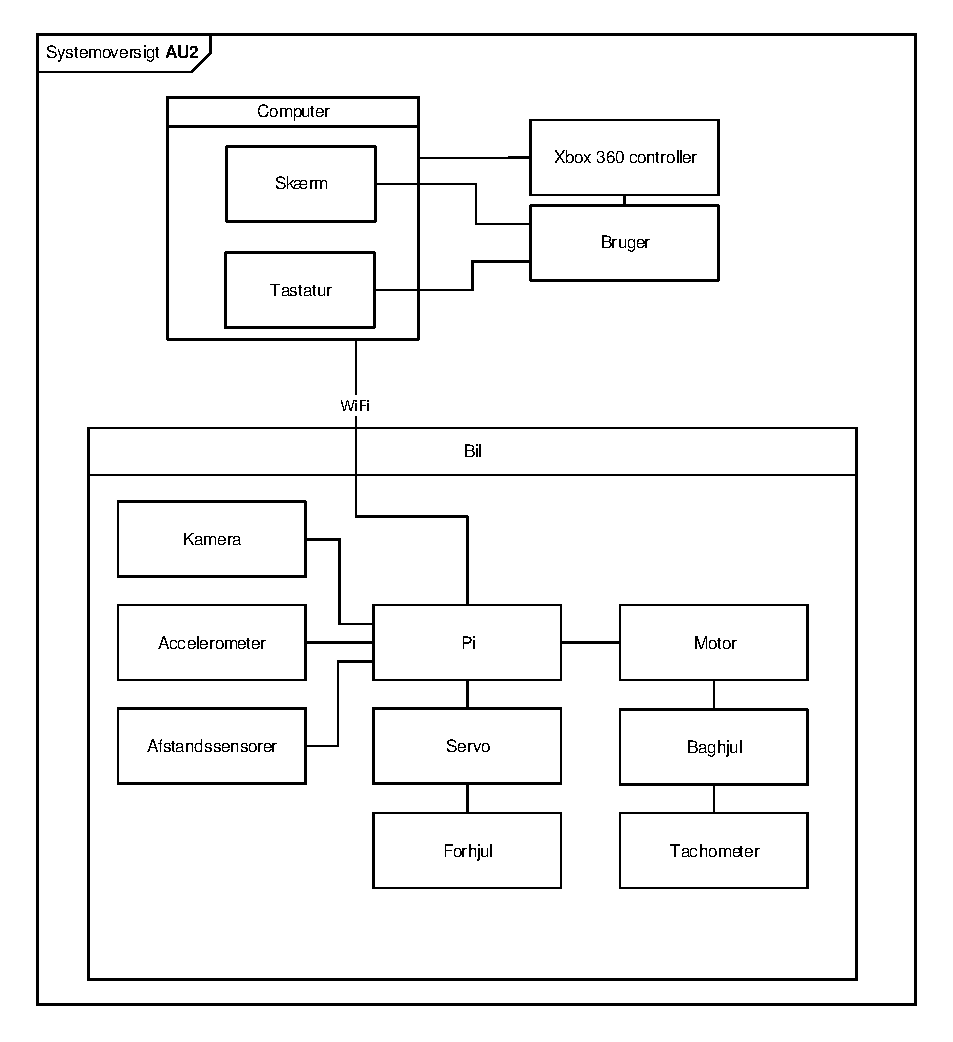
\includegraphics[width=\textwidth * 1]{../fig/diagrammer/systemoversigt}
\caption{Konceptuel oversigt over systemet.}
\label{fig:systmeoversigt}
\end{figure}